
\begin{frame}[fragile]{Un peu de rétro-ingénierie}

La \alert{rétro-ingénierie} consiste à reconstituer un schéma E/A 
à partir d'un schéma relationnel.

\vfill
Intêressant pour comprendre comment une base a été conçue.

\vfill

Intéressant aussi pour maîtriser les rapports entre modélisation conceptuelle
et modélisation relationnelle.

\vfill

\begin{redbullet}
  \item Rétro-ingénierie de la base des immeubles
  \item Introduction d'une entité faible
  \item Introduction d'une réification
\end{redbullet}


\vfill
\begin{blocgauche}
\alert{Ces diapositives correspondent au support en ligne disponible sur
le site \url{http://sql.bdpedia.fr/}}
\end{blocgauche}

\end{frame}


\begin{frame}{Reprenons le schéma de la base des immeubles}


\begin{redbullet}
  \item Immeuble(\textbf{idImmeuble}, nom, adresse)
  \item Appart (\textbf{idAppart}, no , surface , niveau , \textit{idImmeuble})
 \item Personne(\textbf{idPersonne}, prénom, nom, profession, \textit{idAppart})
   \item Propriétaire(\textbf{\textit{idPersonne}, \textit{idAppart}}, quotePart)
\end{redbullet}

\vfill

\begin{blocgauche}
Trouvons les \alert{entités}, les \alert{associations plusieurs-plusieurs},
et pour finir les \alert{associations plusieurs-un}.
\end{blocgauche}
\end{frame}


%%%%%%%%%%%%
\begin{frame}{Le schéma entité-association}


\vfill

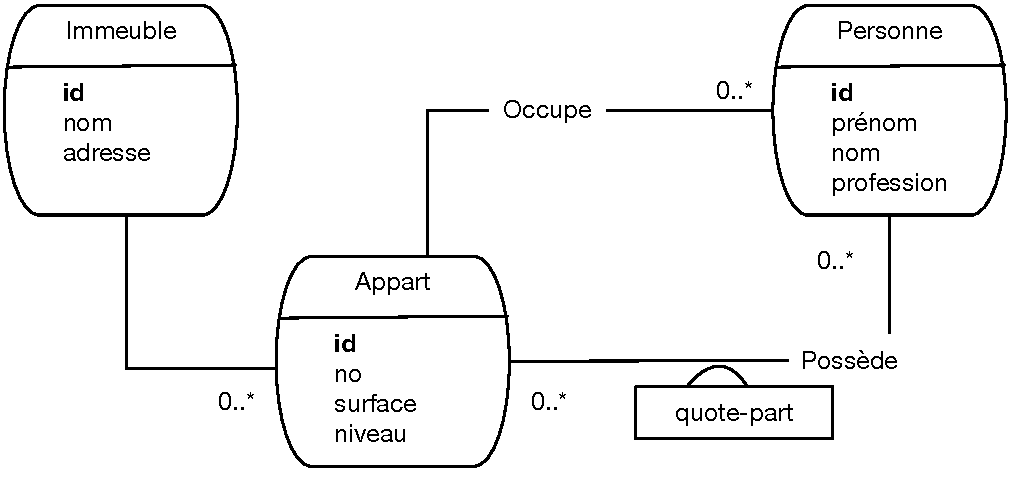
\includegraphics[width=9cm]{../figures-sql/schema-immeubles}

\vfill
\begin{blocgauche}
\alert{Maintenant on peut se poser des questions sur les choix initiaux}
\end{blocgauche}
\end{frame}



%%%%%%%%%%%%
\begin{frame}{Avec entité faible}

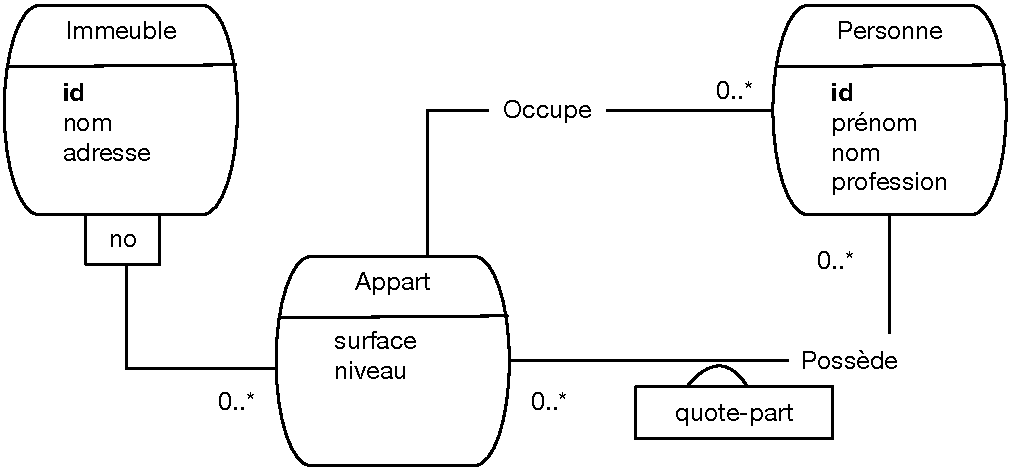
\includegraphics[width=8cm]{../figures-sql/schema-immeubles-avec-faible}

\vfill

\begin{redbullet}
  \item Immeuble(\textbf{idImmeuble}, nom, adresse)
  \item Appart (\textbf{\textit{idImmeuble}, no} , surface , niveau)
 \item Personne(\textbf{idPersonne}, prénom, nom, profession, \textit{idImmeuble, no})
   \item Propriété(\textbf{\textit{idPersonne}, \textit{idImmeuble, no}}, quotePart)
\end{redbullet}

\end{frame}


%%%%%%%%%%%%
\begin{frame}{Avec réification}

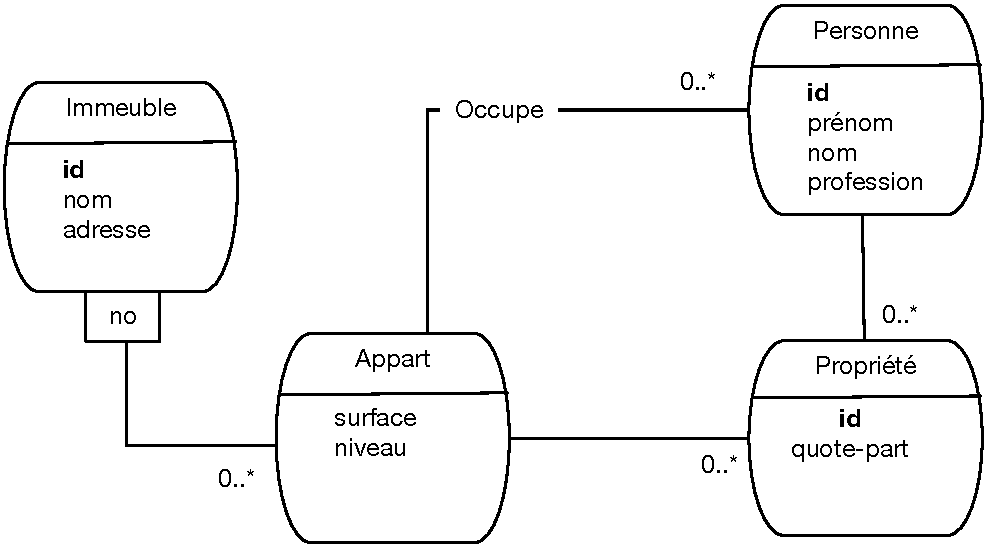
\includegraphics[width=8cm]{../figures-sql/schema-immeubles-reifie}

\vfill

\begin{redbullet}
  \item Immeuble(\textbf{idImmeuble}, nom, adresse)
  \item Appart (\textbf{\textit{idImmeuble}, no} , surface , niveau)
 \item Personne(\textbf{idPersonne}, prénom, nom, profession, \textit{idImmeuble, no})
   \item Propriété(\textbf{id}, \textit{idPersonne}, \textit{idImmeuble, no}, quotePart)
\end{redbullet}

\end{frame}


%%%%%%%%%%%%%
\begin{frame}{À retenir}


Les modélisations entité-association et relationnelle sont très proches l'une
de l'autre.

\vfill

La seule différence est la méthode de représentation des associations\,: 
directe en E/A, indirecte, par clé primaire / clé étrangère, en relationnel.


\vfill
\begin{blocgauche}
Les variantes de modélisation en E/A (typage faible, réification) ont donc
un impact en relationnel sur la représentation des clés, et donc
sur les requêtes des applications\,: \alert{à maîtriser}.
\end{blocgauche}

\end{frame}
